
\documentclass[13pt,compress]{beamer}
% deactivate beamer navigation
%\setbeamertemplate{navigation symbols}{}
%\usepackage{geometry}
%\geometry{papersize={180mm, 135mm}, top=-1.5mm} % 210mm, 297mm

\usepackage[nospeakermargin]{../../style/lmu-lecture}

\setbeamertemplate{frametitle}{\expandafter\uppercase\expandafter\insertframetitle}
%\useoutertheme{metropolis}
% remove section slides
\AtBeginSection[]
{
  \begin{frame}<beamer>
    \frametitle{Supervised Learning II}
    \tableofcontents[currentsection]
  \end{frame}
}
% includepdf slides, pagecommad will set counter for framenumber
\usepackage{pdfpages}
\includepdfset{trim=0mm 0mm 0mm 0mm, pagecommand={\global\setcounter{framenumber}{\value{page}}}}
% trim=0mm 6mm 0mm 0mm, offset=0 15,
% add footer:
\usepackage{framed, color}
\usepackage{xcolor}
%\iffalse
\setbeamertemplate{footline}[text line]{%
    \noindent\hspace*{\dimexpr-\oddsidemargin-1in\relax}%
     \colorbox{white}{
     \makebox[\dimexpr\paperwidth-2\fboxsep\relax]{
     \color{black}
     \begin{minipage}[c][4.5ex][c]{0.5\linewidth}
       \secname
     \end{minipage}
     \hfill\begin{minipage}[c][4.5ex][c]{0.5\linewidth}
       \flushright
       \insertframenumber{}~/~\inserttotalframenumber~~
     \end{minipage}
     }}%
  \hspace*{-\paperwidth}
}
%\fi

\title{Supervised Learning II}
\author{Essential Data Science Training}
%\institute{Essential Data Science Training}
\date{}



\begin{document}
\setbeamercolor{background canvas}{bg=}

% General remark: hyperlinks in included pdfs are not clickable anymore in the combined pdf

\frame{\titlepage}

\section{Classification and Regression Trees}
\includepdf[pages={2-8}, trim=0mm 0mm 45mm 0mm]{../../material/lecture_i2ml/slides-pdf/slides-cart-predictions.pdf}
\includepdf[pages={2-last}, trim=0mm 0mm 45mm 0mm]{../../material/lecture_i2ml/slides-pdf/slides-cart-treegrowing.pdf}
\includepdf[pages={2-7}, trim=0mm 0mm 45mm 0mm]{../../material/lecture_i2ml/slides-pdf/slides-cart-splitcriteria-regression.pdf}
\includepdf[pages={2-4}, trim=0mm 0mm 45mm 0mm]{../../material/lecture_i2ml/slides-pdf/slides-cart-stoppingpruning.pdf}
\includepdf[pages={2-last}, trim=0mm 0mm 45mm 0mm]{../../material/lecture_i2ml/slides-pdf/slides-cart-discussion.pdf}
\section{Random Forest}
\includepdf[pages={2, 4-7}, trim=0mm 0mm 45mm 0mm]{../../material/lecture_i2ml/slides-pdf/slides-forests-nutshell.pdf}
\includepdf[pages={2-last}, trim=0mm 0mm 45mm 0mm]{../../material/lecture_i2ml/slides-pdf/slides-forests-benchmark.pdf}
\includepdf[pages={2-3}, trim=0mm 0mm 45mm 0mm]{../../material/lecture_i2ml/slides-pdf/slides-forests-discussion.pdf}
\section{Exercise: Tree methods with mlr3}
\begin{frame}{Exercise: Tree methods with mlr3}
File: \textit{day2\_tree\_methods.html}
\end{frame}
\section{Tuning}
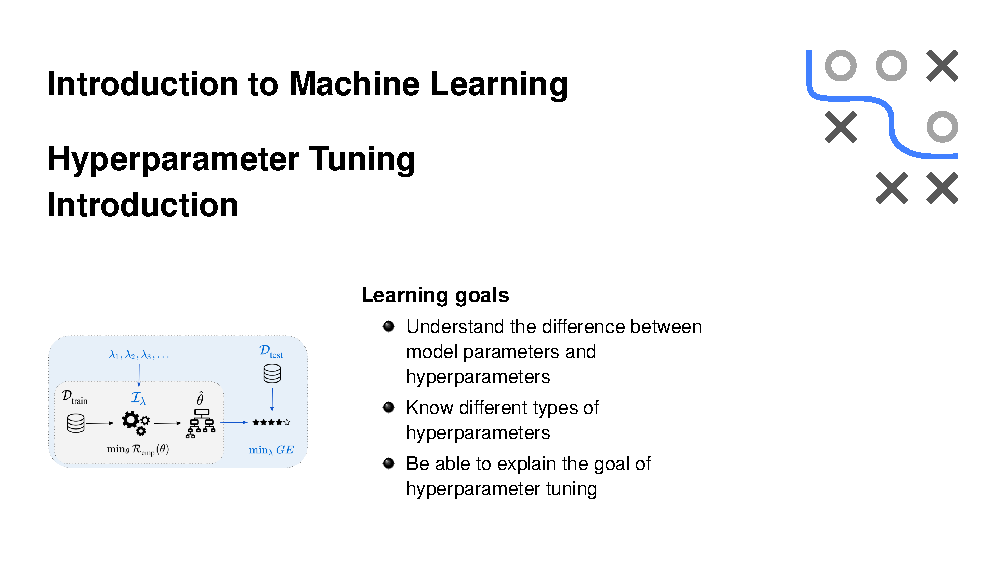
\includepdf[pages={1-last}, trim=0mm 0mm 45mm 0mm]{../../material/lecture_i2ml/slides-pdf/slides-tuning-intro.pdf}
\includepdf[pages={2-3, 5-last}, trim=0mm 0mm 45mm 0mm]{../../material/lecture_i2ml/slides-pdf/slides-tuning-tuningproblem.pdf}
\includepdf[pages={2-last}, trim=0mm 0mm 45mm 0mm]{../../material/lecture_i2ml/slides-pdf/slides-tuning-basicalgos.pdf}
\section{Tuning with mlr3tuning}
\includepdf[pages={3-4, 8, 11, 13, 15, 16, 18, 21, 24, 29-33, 35-39}]{../../material/mlr-doc/CURRENT_mlr3_course/02_mlr3tuning/mlr3tuning.pdf}
\section{Exercise: Tuning with mlr3tuning}
\begin{frame}{Exercise: Tuning with mlr3tuning}
File: \textit{day2\_tuning.html}
\end{frame}
\section{Nested Resampling}
\includepdf[pages={2-last}, trim=0mm 0mm 45mm 0mm]{../../material/lecture_i2ml/slides-pdf/slides-nested-trainvalidtest.pdf}
\includepdf[pages={2-6}, trim=0mm 0mm 45mm 0mm]{../../material/lecture_i2ml/slides-pdf/slides-nested-nestedresampling.pdf}
\section{Nested Resampling with mlr3tuning}
\includepdf[pages={51-last}]{../../material/mlr-doc/CURRENT_mlr3_course/02_mlr3tuning/mlr3tuning.pdf}
\section{Exercise: Nested Resampling with mlr3tuning}
\begin{frame}{Exercise: Nested Resampling with mlr3tuning}
File: \textit{day2\_nested\_resampling.html}
\end{frame}
\section{Regularization}
\includepdf[pages={3-5, 11-12, 14-16}]{../../material/lecture_i2ml/slides-pdf/slides-regu-intro.pdf}
\includepdf[pages={2-3, 8}]{../../material/lecture_i2ml/slides-pdf/slides-regu-l1l2.pdf}
\includepdf[pages={2, 8-9}]{../../material/lecture_i2ml/slides-pdf/slides-regu-l1vsl2.pdf}
\includepdf[pages={2}]{../../material/lecture_i2ml/slides-pdf/slides-regu-enetlogreg.pdf}
\includepdf[pages={2-5, 7-8}]{../../material/lecture_i2ml/slides-pdf/slides-regu-nonlin-bayes.pdf}
\section{Appendix: Advanced Tuning}
\includepdf[pages={2, 4-10, 15}, trim=0mm 0mm 45mm 0mm]{../../material/lecture_i2ml/slides-pdf/slides-tuning-advanced.pdf}



\end{document}
